\section{Reimplementation Strategy}
\label{sec:remplementation}

The main purpose of my implementation work was to be able to code by myself some of the core ideas of the ADOP differentiable point based neural renderer.
I decided to code everything from scratch knowing since the start that I would at no point be able to fully reproduce the results from the authors but I learnt a large amount of things by doing so.
\begin{itemize}
    \item I used BlenderProc \cite{Denninger2023} to script and generate multiple synthetic scenes from the samples used in the NerF paper. All camera positions are known and share the same referential as my pytorch point renderer.
    \item A perfect point cloud is sampled at random from the mesh (through the .obj file).
    \item A few pytorch based function allows to project the points onto the image plane and include soft depth test and normal culling.
    \item A CNN is trained to predict the right dense color of the points in the image space.
\end{itemize}

Each element has been carefully tested by mostly visual tests.
Below is the list of all simplifications that have been made compared to the original ADOP paper.
\begin{itemize}
    \item We assume linear RGB cameras without tone mappings.
    \item We discard environment map (e.g. our background is black).
    \item We generate photorealistic renders of synthetic meshes instead of using real photos. 
    \item Camera poses are perfectly known.
    \item We do not refine the camera poses (no need to be approximately differentiable with regard to camera geometry parameters).
    \item Using meshes allows us sampling point clouds with normals without estimation errors such as the one we'd face with COLMAP.
    \item We can easily control the number of points to be able to test on a limited capacity GPU with only 4Gb of RAM.
\end{itemize}

\begin{figure}[H]
    \centering
    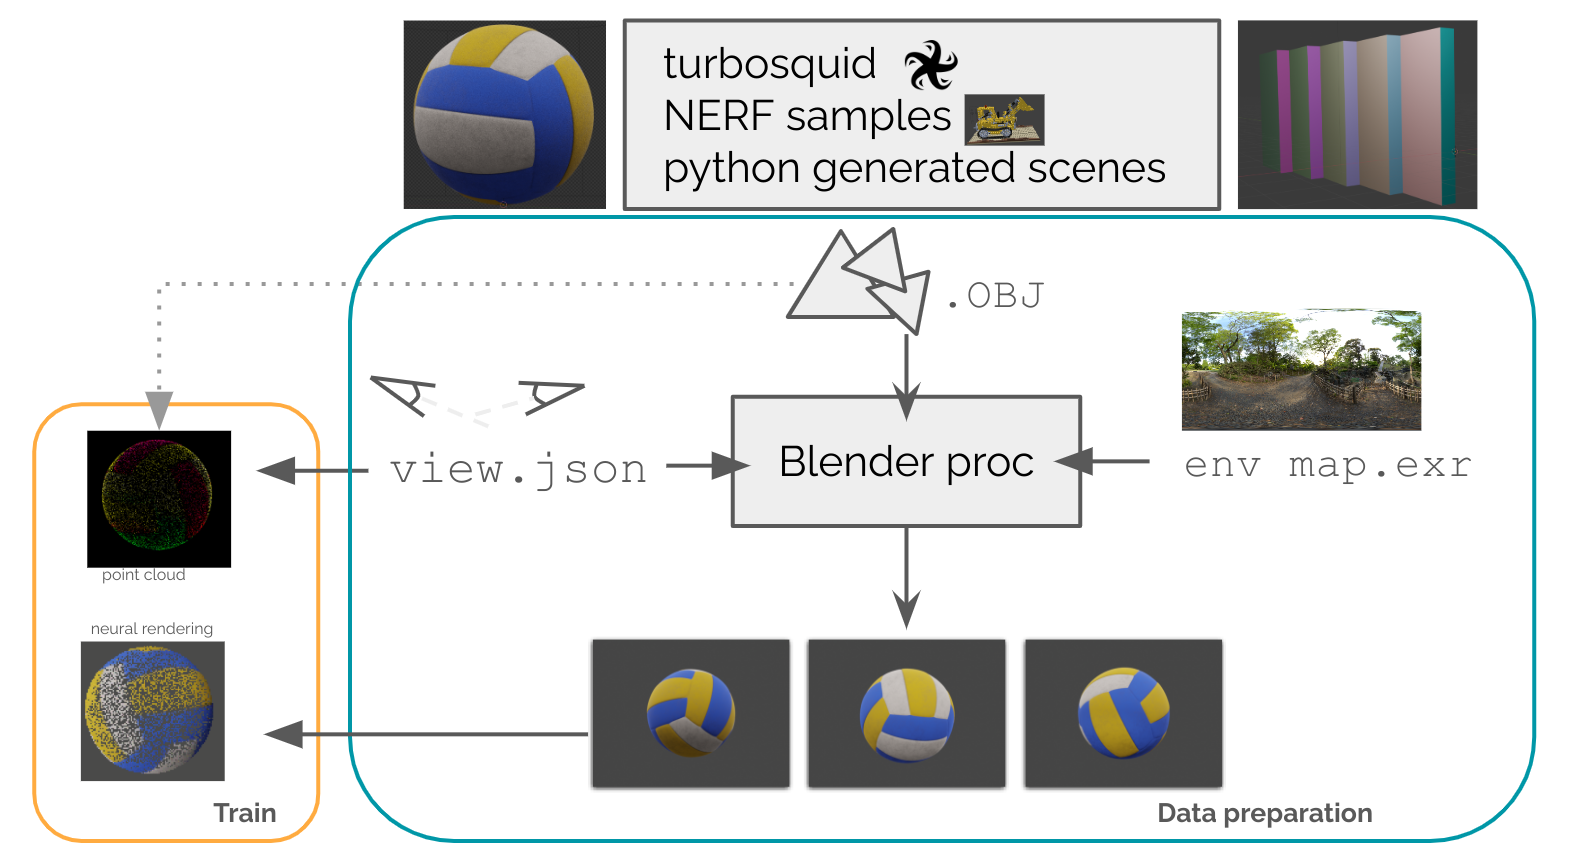
\includegraphics[width=0.5\textwidth]{figures/data_prep_and_training.png}
    \caption{Workflow: \href{https://github.com/balthazarneveu/per-pixel-point-rendering/blob/main/studies/photorealistic\_rendering.py}{\texttt{photorealistic\_rendering.py}} allows preparing camera multiviews positions saved as \texttt{.json} files in order to render photorealistic views of a \texttt{.blend} or  \texttt{.obj} files which come from internet resources or test scenes generated in python.
    The .obj and view .json files tie together the BlenderProc rendering and my Pytorch point rendering implementation: The point cloud is sampled from the mesh and the camera poses are known. A neural network is trained using \href{https://github.com/balthazarneveu/per-pixel-point-rendering/blob/main/scripts/optimize\_point\_based\_neural\_renderer.py}{\texttt{optimize\_point\_based\_neural\_renderer.py}} to predict colors of the points by trying to match the multiple photorealistic renderings. CNN weights, pointcloud, normals and pseudo-colors are all saved along in a \texttt{.pt} file which later allows performing live novel view synthesis \href{https://github.com/balthazarneveu/per-pixel-point-rendering/blob/main/scripts/novel\_views\_interactive.py}{\texttt{novel\_views\_interactive.py}} based on the self developped \href{https://github.com/balthazarneveu/interactive\_pipe}{interactive\_pipe} library}.
    \label{fig:data_and_train}
\end{figure}


\subsection{Generating synthetic calibrated scenes}
\label{sec:synthetic_calibrated_scenes}
In order to avoid dealing with large real scenes with millions of points and having to deal with heavy COLMAP processing, I decided to use a recent library named BlenderProc  \cite{Denninger2023} which simplifies the use of Blender as it allows running renders in the background (launched through terminal without the need of a graphical user interface).

It is first possible to generate a set of viewpoints configurations to orbit around the scene. It is also possible to generate an environment map (e.g. a skybox). We render with the background transparency option so the rendering results is a RGB PNG. 
% 1532.9s for 60 views of the \texttt{material balls}.
% 753.869 ficus

% Rendering is peformed using GPU and requires 25 seconds per view with a resolution 640x480 for the \texttt{material balls}. scene on a laptop Nvidia T500.
% 27 minutes are needed to generate 64 viewpoints
\begin{figure}[H]
    \centering
    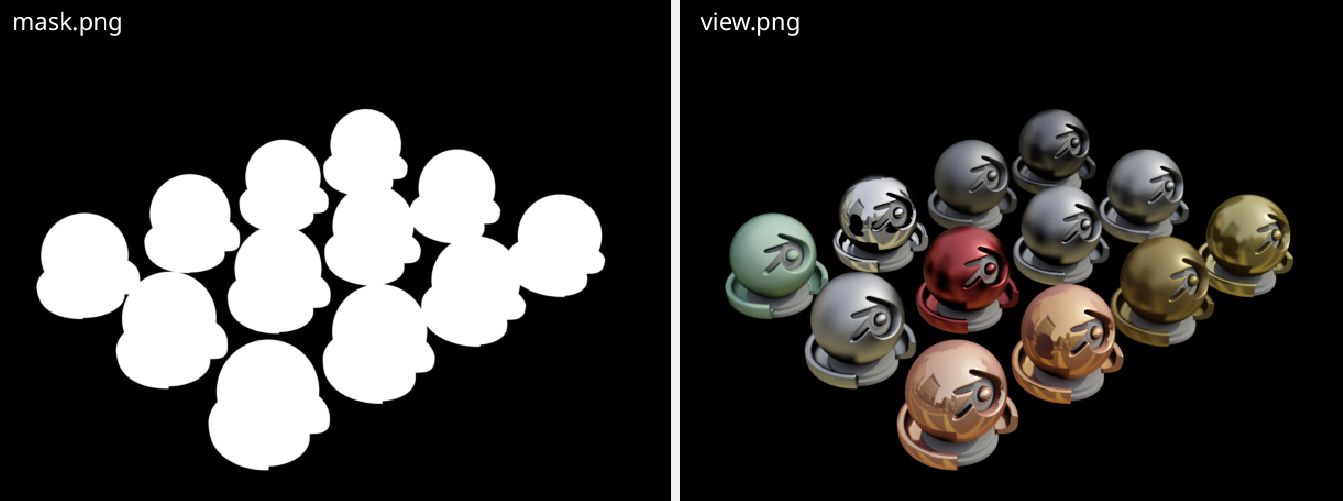
\includegraphics[width=0.5\textwidth]{figures/blenderproc_renders.png}
    \caption{Mask and RGB render BlenderProc renders with an environment map.}
    \label{fig:blenderproc_renders}
\end{figure}

\begin{figure}[H]
    \centering
    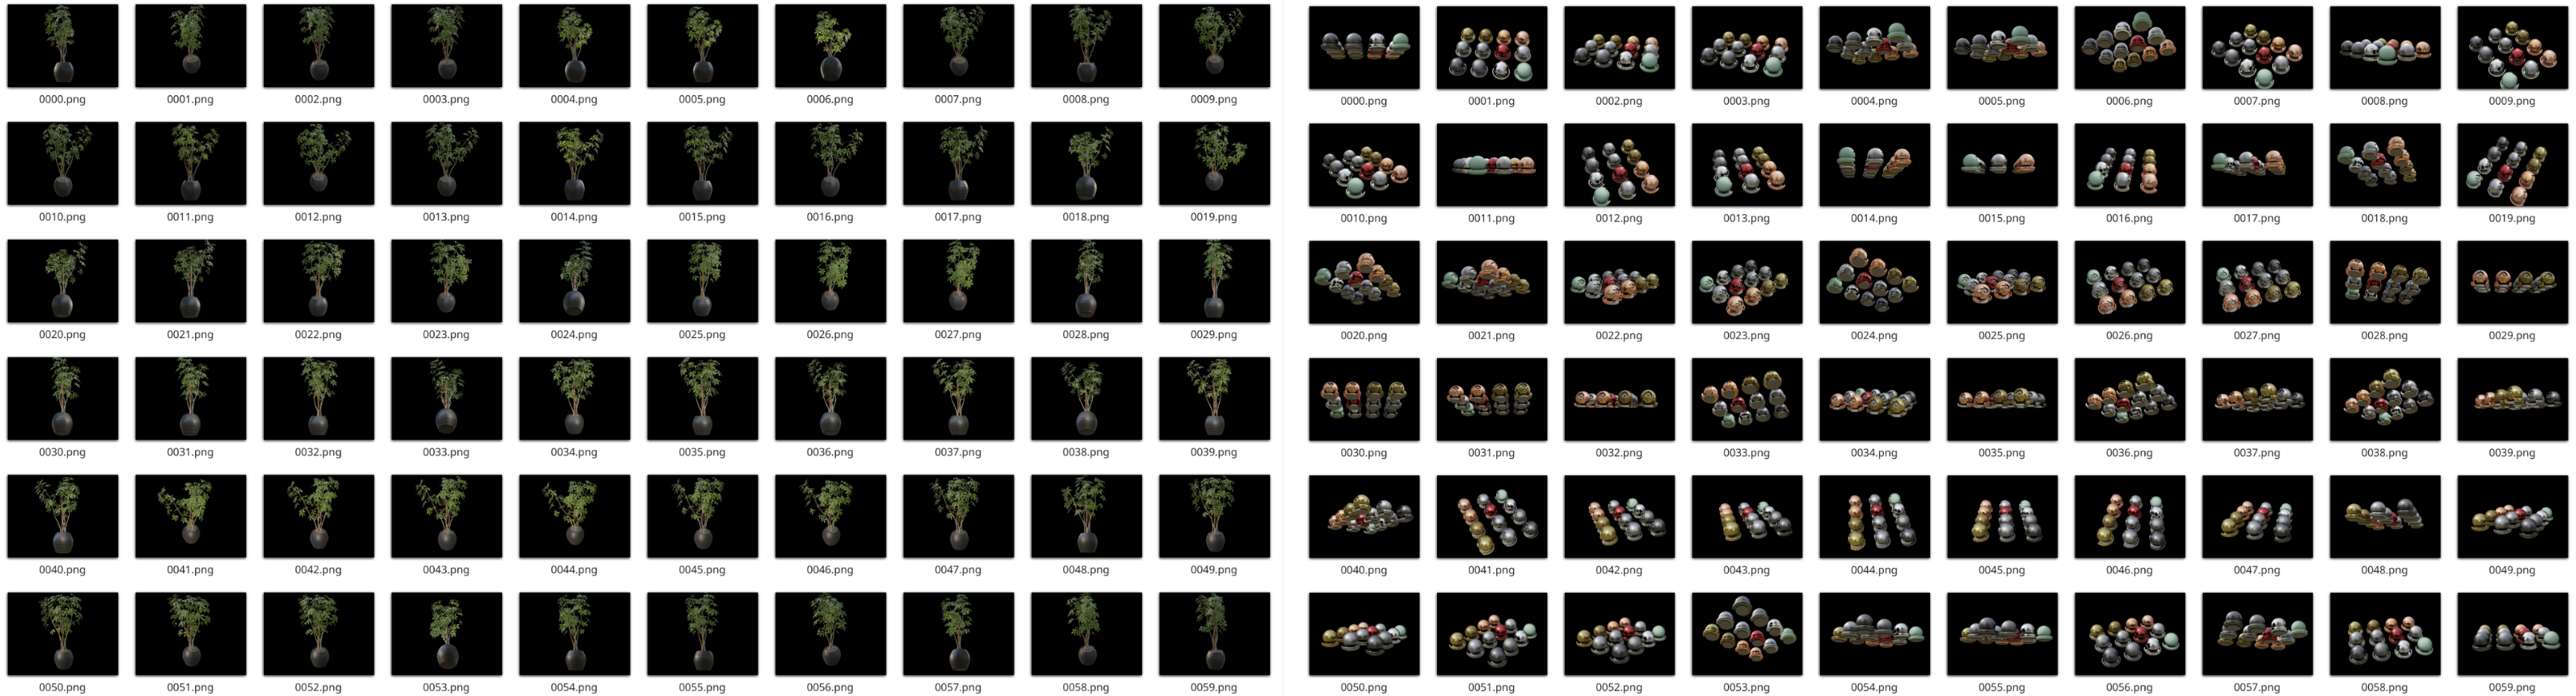
\includegraphics[width=0.5\textwidth]{figures/ficus_and_matballs.png}
    \caption{60 views of resolution 640x480 of the \texttt{Ficus} scene rendered in 12 minutes On the right, \texttt{material balls} scene rendered in a total of 25 minutes on a laptop equipped with a Nvidia T500.}
    \label{fig:multiview}
\end{figure}

Using the environment map as a background has been disabled in BlenderProc as it allows to simplify and remove one of the extra components of the ADOP paper (e.g. it allows rendering the point cloud without using the neural environment map trick and we use black uniform color instead).

We parameterize camera orientation using 3 Euler Angles (yaw pitch roll) and 3 positions. We build the extrinsic camera matrix from the 3 angles and use a pinhole camera model to project 3D points onto the image plane as we'll see in ~\cref{sec:projecting_the_point_cloud_onto_the_image_plane}. There's a perfect equivalence between the camera parameters used in Blender and the ones used in my Pytorch renderer.

One of the difficulties of using synthetic rendering from meshes is that sometimes thin surfaces are modeled with double sided triangles. Since our rendering pipeline is using normal culling, we end up with an issue: points with normals not pointing towards the camera are not rendered. So on the ficus scene for instance, if we look "at the green leafs" from the bottom, the green leaves will become transparent so the renderer will have a hard time during reconstruction. We may therefore stick to objects with easy geometry such as the \texttt{old chair} scene. This is illustrated in \cref{fig:ficus_culling_issue}.

When working on natural scenes, the points will most probably be duplicated on both sides of the surface by COLMAP with the normals in both ways. In my case, I sampling points randomly from the mesh and I simply take the normal of the triangle to which the point belongs without considering it double sided.

I first notticed this effect on my synthetic \texttt{stair case} scene which was only made of planes and that could not be optimized in the trivial "Bypass" case.

\begin{figure*}
    \centering
    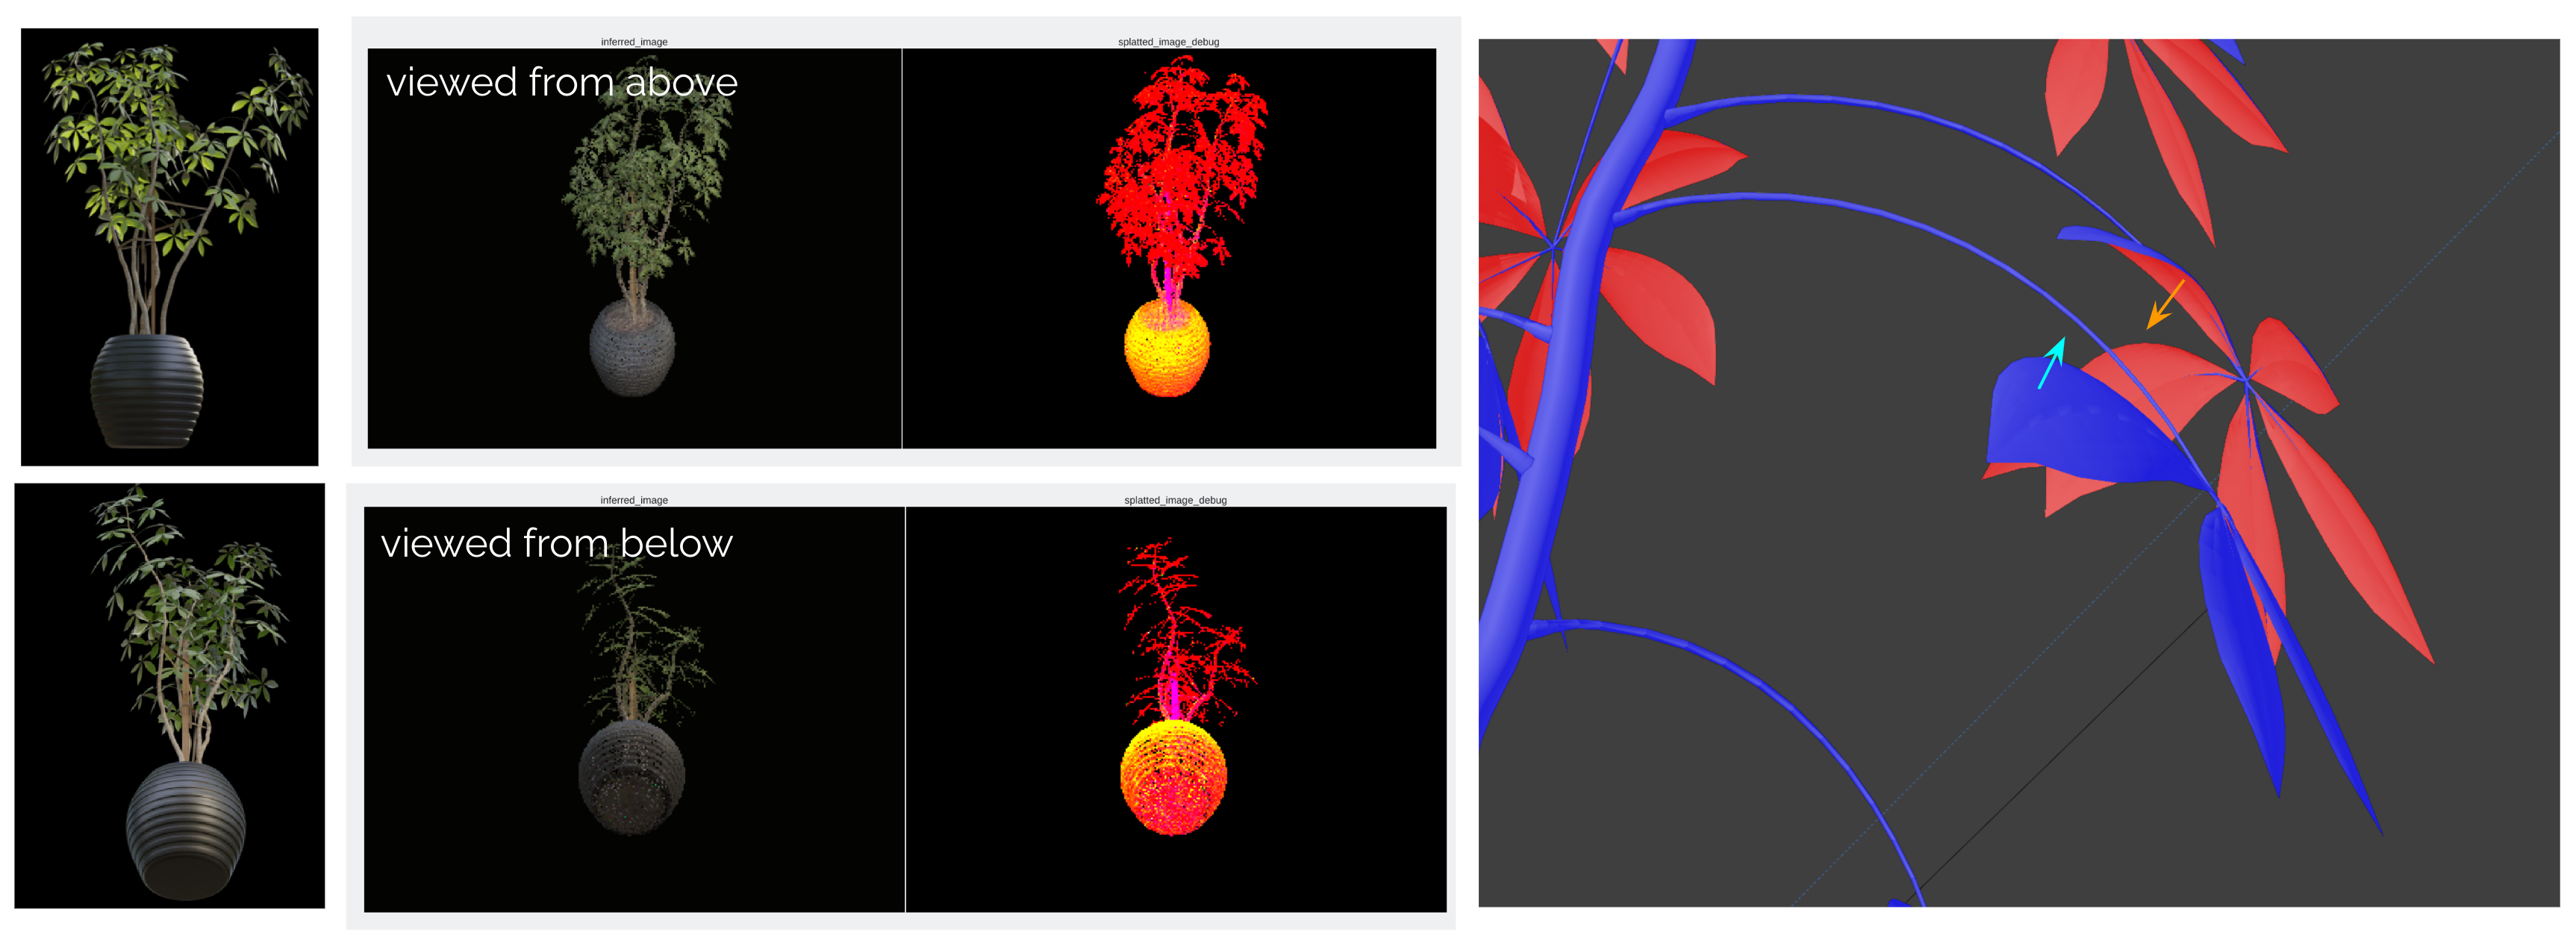
\includegraphics[width=0.8\textwidth]{figures/double_sided_surfaces_issues.png}
    \caption{On the left, image from the Blender render of the ficus scene, seen slightly from below where the leaves look brighter than when looked from above. On the right side, we check the rendering of the point cloud with the "Bypass" mode (which allows ajusting the colors points to the scene). Most leaves are oriented upwards so normal culling does not render these points when seen from below. The optimization process has trouble to reconstruct correct colors for the leaves. On the right side, the blender face orientation (blue front facing the camera/red back facing the camera) fully reveals that the leaves of the \texttt{ficus} scene are made of double sided triangles.}
    \label{fig:ficus_culling_issue}
\end{figure*}

\subsection{Projecting the point cloud onto the image plane}
\label{sec:projecting_the_point_cloud_onto_the_image_plane}

\subsubsection{Coordinates projection}
\label{sec:coordinates_projection}

\begin{figure}[H]
    \centering
    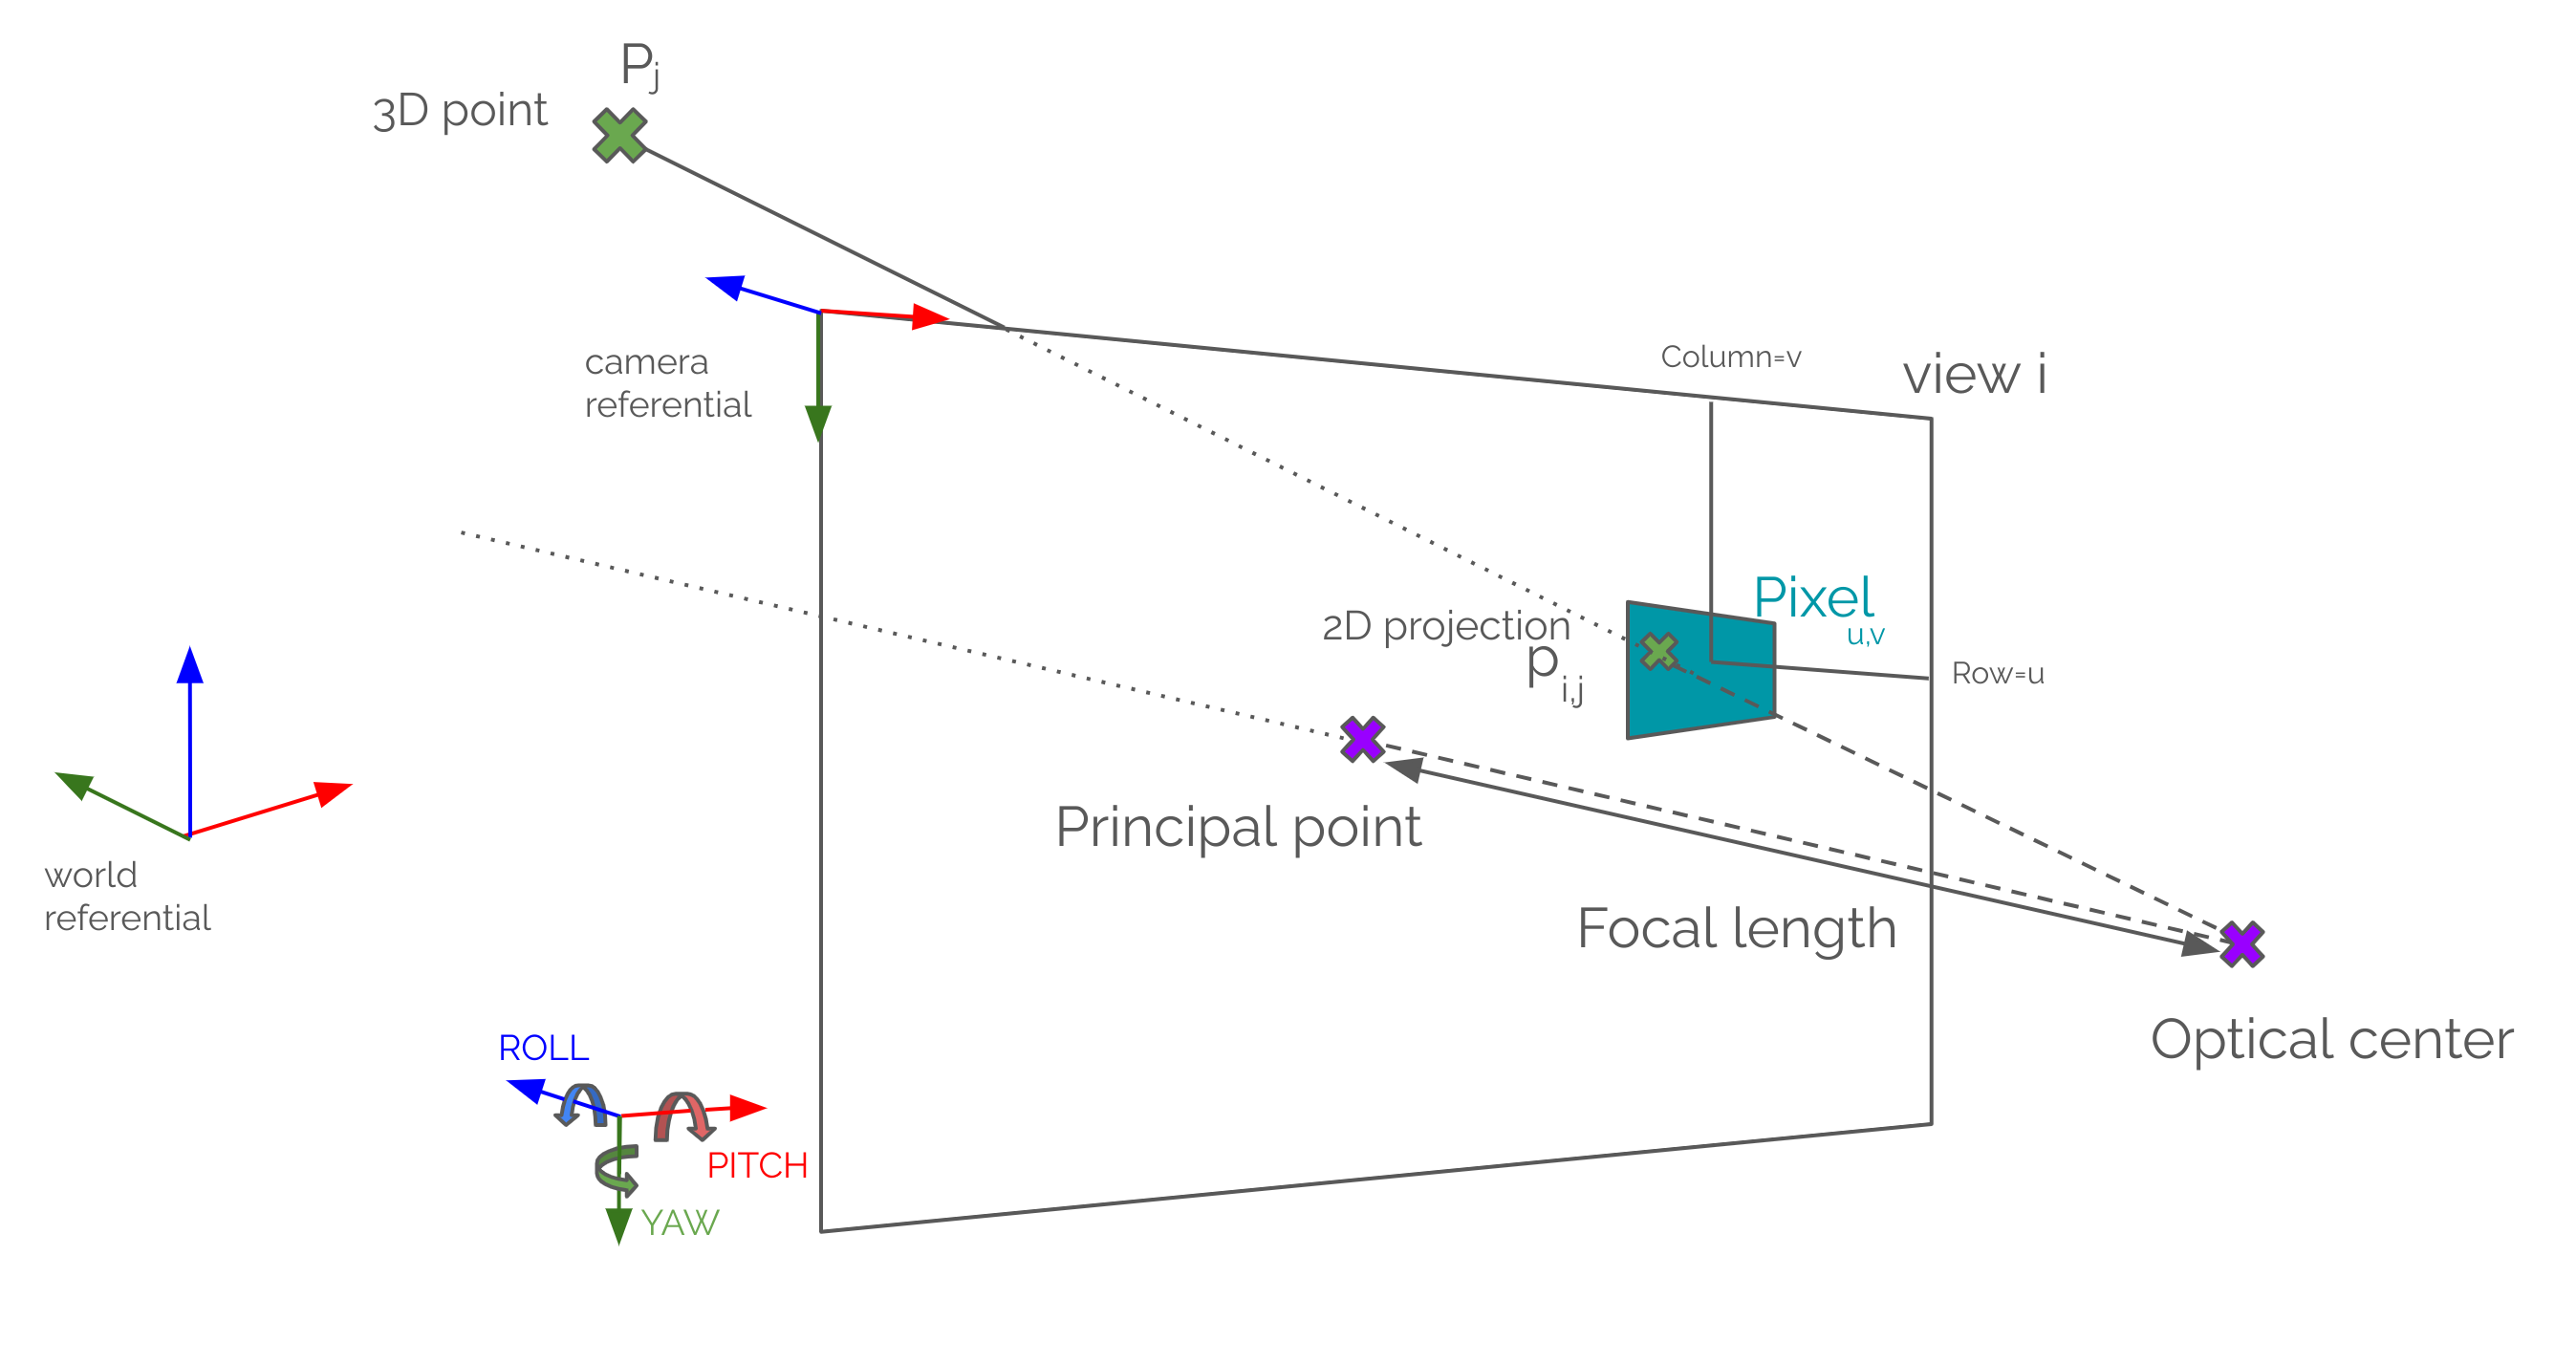
\includegraphics[width=0.4\textwidth]{figures/pinhole_camera_with_angles.png}
    \caption{Pinhole camera model. The $j^\text{th}$ point of the 3D point cloud, located at $\vec{P_{\textrm{3D}}}^{(j)}$ expressed in world coordinates is projected onto the sensor plane for view $i$ at position $\vec{p_{\textrm{2D}}}^{(i,j)}$ expressed as pixel coordinates, rounded to the 2D nearest integer coordinates $(u,v)$}
    \label{fig:pinhole_camera}
\end{figure}


To project a 3D point of index $j$ located at $\vec{P_{\textrm{3D}}}^{(j)}$ in world coordinates onto the image sensor,
we use the pinhole projection model as illustrated in \ref{fig:pinhole_camera}.

$$\vec{p_{\textrm{2D}}}^{(j)} = K\cdot\left[Q_{\text{cam}} | T_{\text{cam}}\right]^{i}\vec{P_{\textrm{3D}}}^{(j)}$$
where
\begin{itemize}
    \item $K$ is the camera 3x3 intrinsic matrix.
    \item $Q_{\textrm{cam}}^{i}$ is the camera orientation for view $i$, this matrix is created from the yaw, pitch, roll angles.
    \item $T_{\textrm{cam}}^{i}$ is the 3D camera position for view $i$ in the world frame (meters)
    \item $\vec{P_{\textrm{3D}}}^{(j)} \in \mathbb{R}^{4}$ are the homogeneous 3D coordinates of point $j$ in the world frame.
    \item $\vec{p_{\textrm{2D}}}^{(i,j)} \in \mathbb{R}^{3}$ are the homogeneous 2D coordinates of point $j$ projected in the sensor frame $i$ (pixel coordinates).
\end{itemize}

This operation is performed in ~\href{https://github.com/balthazarneveu/per-pixel-point-rendering/blob/main/src/pixr/rendering/forward_project.py}{\texttt{forward\_project.py}} in parallel over all points $j$ , using \texttt{torch.matmul} operation

\noindent \textit{Points coordinates could probably be projected all at once for all camera views using \texttt{torch.bmm}.}


\noindent \textbf{Multiscale.} Pseudocolored projected point cloud will be rendered at multiple scales. For a given scale $l \in \{0, 1, 2, 3\}$, 
$(u,v)^{(l)}$ are the rounded coordinates version of $\frac{\vec{p_{\textrm{2D}}}^{(i,j)}}{2^{l}}$.

\subsubsection{Scatter operation.}
\label{sec:scatter_op}

Visible points's colors are copied into corresponding pixels on the 2D image. A point only leads to a single pixel color update by taking the nearest pixel coordinate of $\lceil\vec{p_{\textrm{2D}}}^{(j)}\rfloor$. There are conditions to satisfy for each point to be valid. 
\begin{itemize}
    \item $(C1)$ The point must be inside the image frame $0\leq x<W$ and $0\leq y <H$.
    \item $(C2)$ The point must be in front of the camera ($Z>0$).
    \item $(C3)$ The normal of the point must face the camera - see ~\cref{fig:normal_culling_validation}.
    \item $(C4)$ The point must not be occluded by another point.
\end{itemize}

\begin{figure}[htpb]
    \centering
    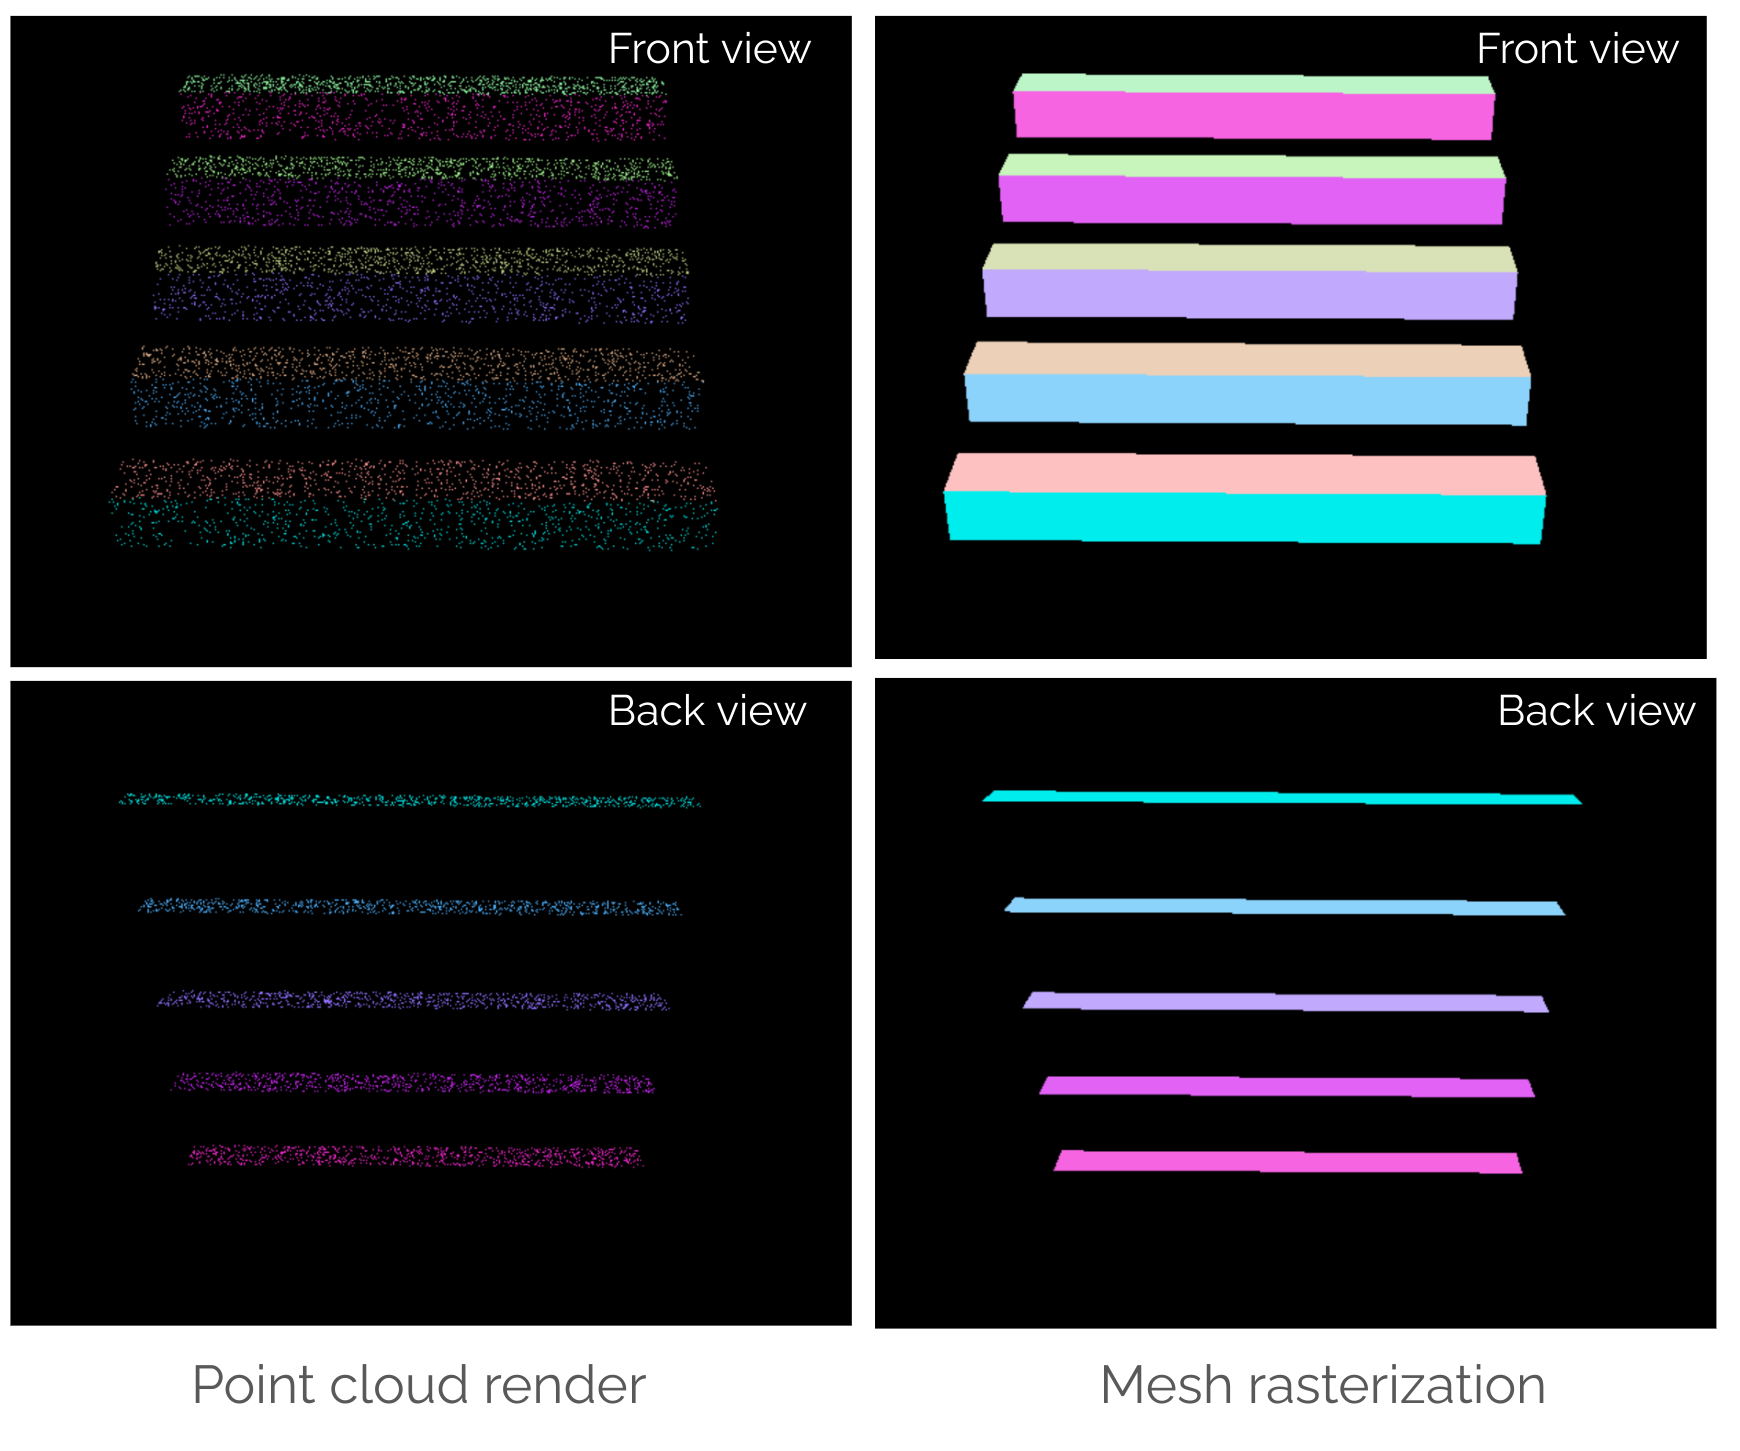
\includegraphics[width=0.45\textwidth]{figures/normal_culling_validation.png}
    \caption{Validation of normal culling. We do not render points with normals pointing away from the camera.}
    \label{fig:normal_culling_validation}
\end{figure}



\noindent \textbf{Soft depth test.} 
That last condition requires some work:
Using a Z-buffer, it is possible to take the closest point to the camera. Since several points may fall into the same pixel cell, there will be aliasing as several pixels may be located on the same suface. The authors rely on previous work \cite{schutz2021rendering} to average point colors in a tiny range of depths located behind the closest point. This is called a soft depth test and we'll describe this part in details as it required a tricky implementation with Pytorch.

\begin{figure}[H]
    \centering
    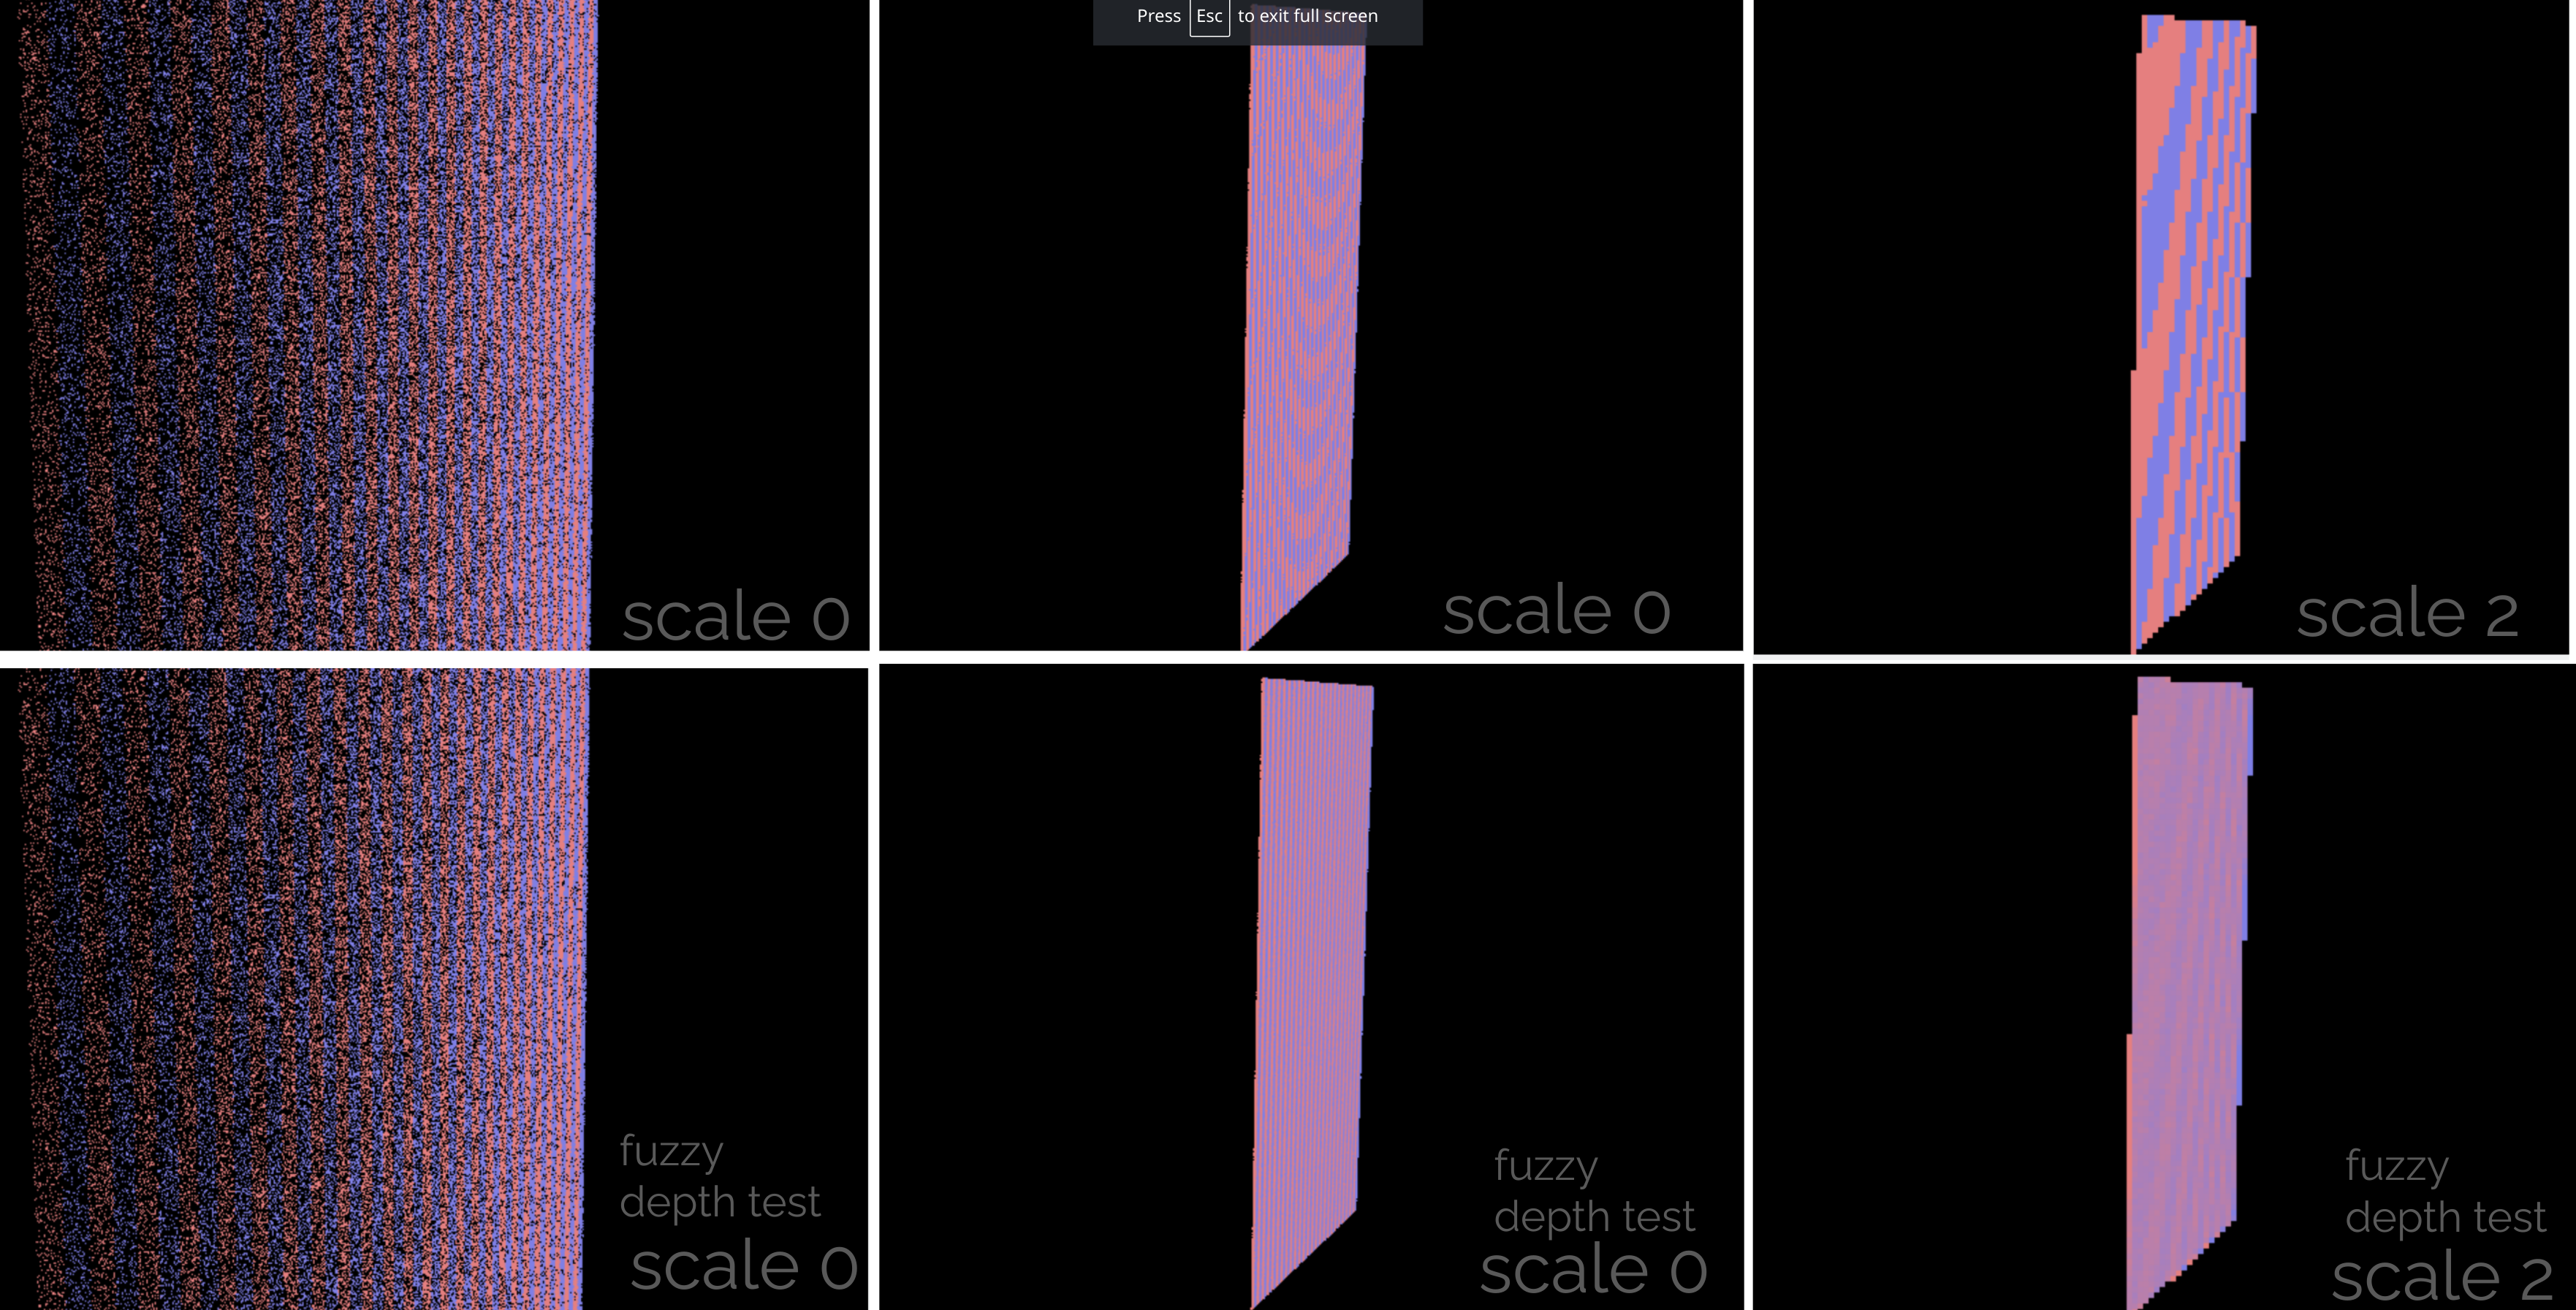
\includegraphics[width=0.45\textwidth]{figures/fuzzy_depth_test_aliasing_large.png}
    \caption{Fuzzy depth test acts as an anti-aliasing filter. On this test scene, a point cloud made of 500.000 point located in the same plane with an alternate vertical red an blue stripes on . We use $\alpha=0$ on the top (hard depth test) and $\alpha=0.01$ on the bottom (soft depth test). On the right side, when using larger scales (lower resolutions), aliasing effect if naturally amplified.}
    \label{fig:fuzzy_depth_test_AA}
\end{figure}

Soft depth test $Z \leq (1 + \alpha) * \textrm{min}_{Z_{j}}$ requires two passes. First compute the closest point to the camera for each pixel. Then, for each pixel, average the colors of the points that are close enough to the closest point. As we'll perform the first pass, we'll keep track of conditions $(C1)$, $(C2)$ and $(C3)$ to avoid recomputing them during the second pass.

\noindent \textbf{First pass: Hard depth test.}

\noindent ~\href{https://github.com/balthazarneveu/per-pixel-point-rendering/blob/main/src/pixr/rendering/zbuffer\_pass.py#L5}{\texttt{zbuffer\_pass.py}} is the first pass. It allows to find the closest point to the camera for each pixel. Depth values are initialized at $\inf$ and will remain $\inf$ when a pixel has not been filled. A first implementation trick is for each point of index $j$ to keep a linear index $k$ of its coordinate position in the image $k[j] = 1+ u*W+v$ if the point is valid regarding conditions $(C1)$, $(C2)$ and $(C3)$ and set this index to $k[j]=0$ otherwise. This allows to avoid recomputing the same test conditions during the second pass.

We then obtain the closest depth image for each pixel. $\forall (u,v) \in \left[0, H-1\right] \times \left[0, W-1\right]$:
$$Z^{\texttt{min}}_{(u,v)} = min_{\left\{j  \text{ s.t. } k[j]=1+u*W+v\right\}} \left(Z[j]\right)$$
\noindent Although this index mapping looks unnatural, it allows to use the ~\href{https://pytorch.org/docs/stable/generated/torch.Tensor.scatter\_reduce\_.html#torch.Tensor.scatter\_reduce\_}{\texttt{torch.scatter\_reduce\_}} operation to take the minimum of depth values for each pixel in a 1D tensor of size $1+W*H$.

My first ~\href{https://github.com/balthazarneveu/per-pixel-point-rendering/blob/main/src/pixr/rendering/legacy\_splatting.py}{\texttt{legacy\_splatting.py} implementation with a for loop} was way too slow and using native torch operators allowed me to get fast point cloud rendering (and save some development time to avoid rewriting a custom CUDA kernel).

\noindent \textbf{Second pass. Soft depth test and color aggregation}

In the second pass  ~\href{https://github.com/balthazarneveu/per-pixel-point-rendering/blob/main/src/pixr/rendering/colors\_aggregation.py}{rendering/colors\_aggregation.py}, we are now capable to apply the soft depth test as we have already computed the closest distance of the point cloud to the camera for each pixel. We'll modify the point index mapping $k[i]$ to only keep indices which satisfy the soft depth test: 
$$ k'[j] = k[j] * \left(Z[j] \leq (1+\alpha) *Z^{\texttt{min}}_{(u,v) \equiv k[j]}\right)$$

\noindent Multiplying by the boolean tensor gracefully sets to 0 the indices which do not satisfy the condition and keeps the others unchanged. Keep in mind that the $k=0$ index is the invalid pixel and will be discarded.
Finally, we average the colors of the points that satisfy the soft depth test, at each pixel location, using \texttt{torch.scatter\_reduce\_} operator with the \texttt{reduce=`mean`}. It is possible to keep a background

\begin{figure*}[h]
    \centering
    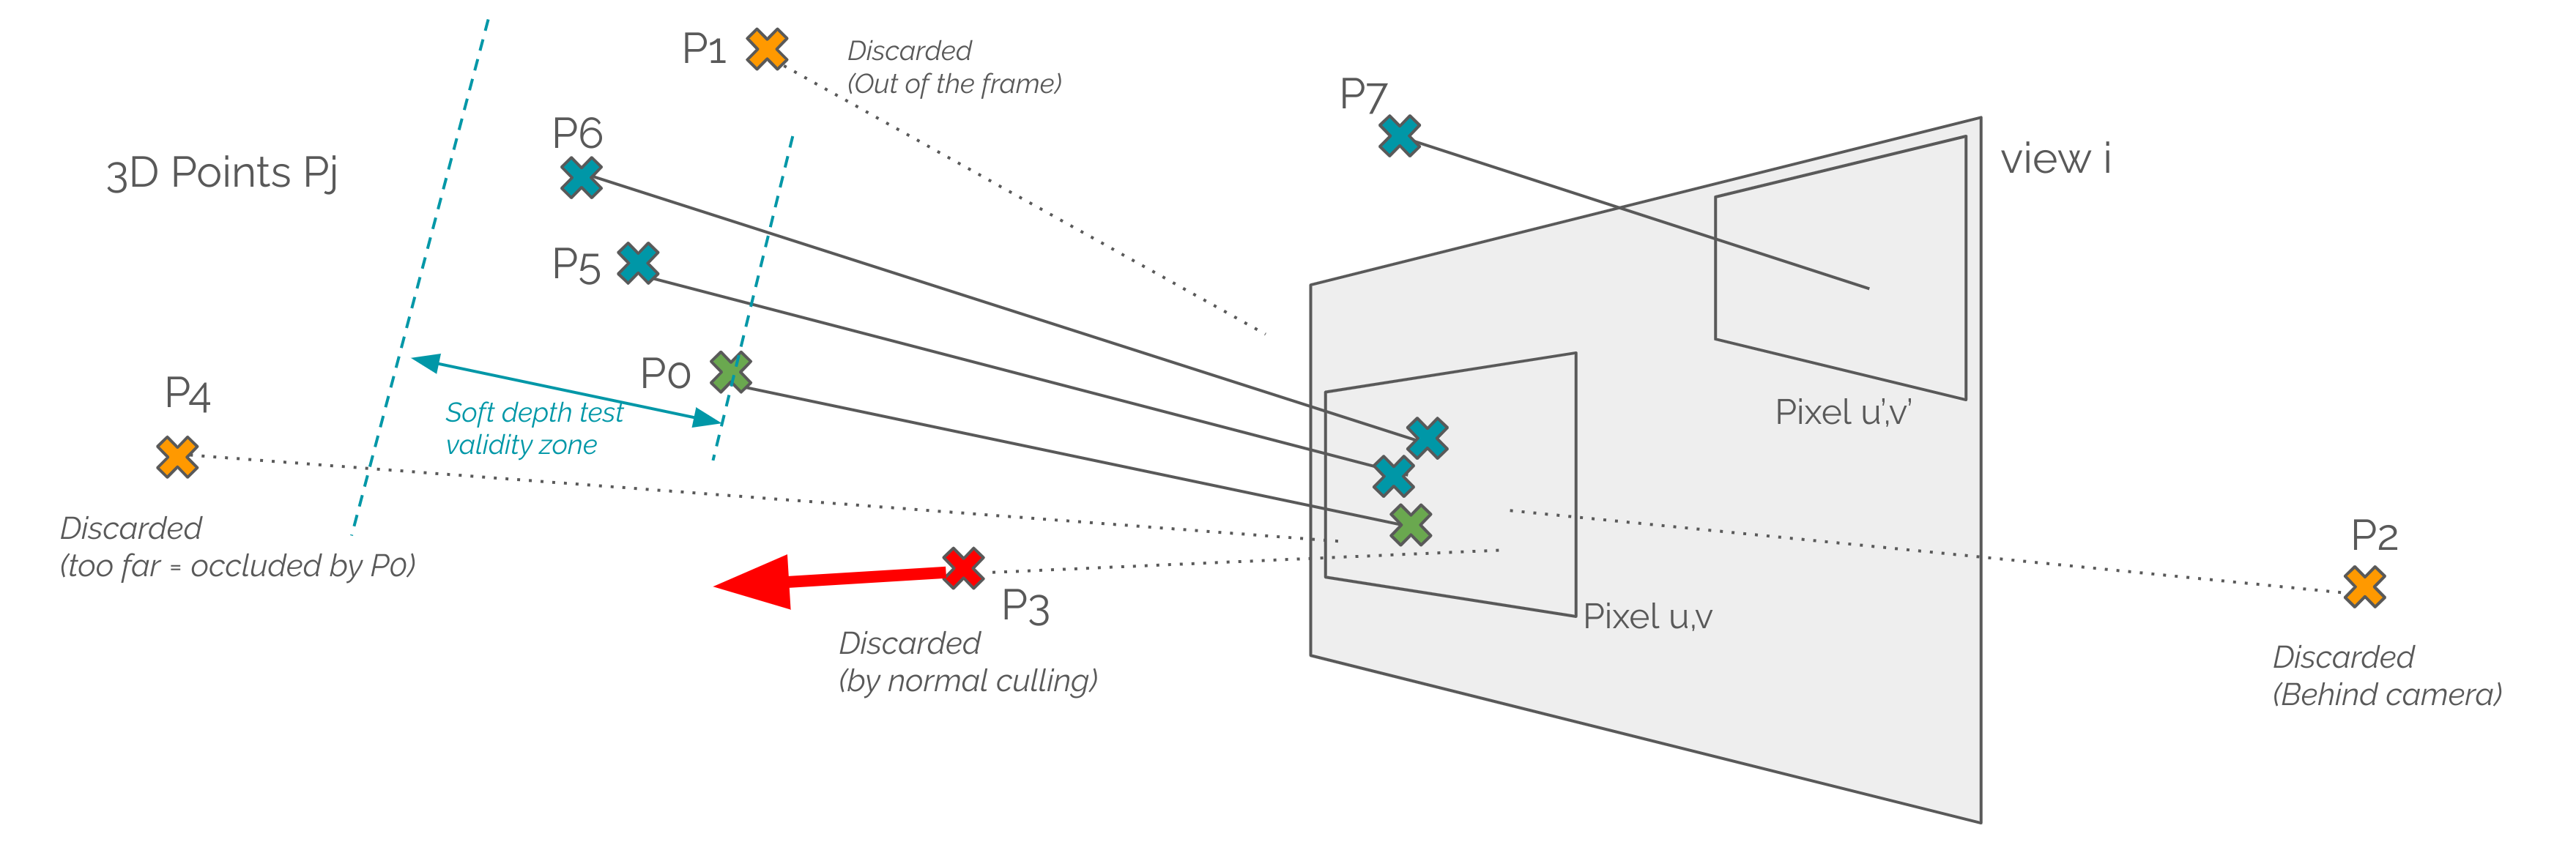
\includegraphics[width=0.9\textwidth]{figures/soft_depth_test_two_pixels.png}
    \caption{Soft depth test illustration: 
    $P^{(0)}$ is the closest point to the camera for pixel $(u,v)$. We will average the colors of the points $(P^{(0)}, P^{(5)}, P^{(6)})$. During the first pass, we'll keep track of the mapping between point indices and projected coordinates (in a 1D fashion). $k[0]=k[4]=k[5]=k[6]=1+u*W+v$ and $k[1]=k[2]=k[3]=0$, $k[7] = 1+u'*W+v'$. First pass will find the minimum of depths for each pixel $Z^{\texttt{min}}_{(u,v)} = min_{\left\{j  \text{ s.t. } k[j]=1+u*W+v\right\}} \left(Z[j]\right), \forall (u,v) \in \left[0, H-1\right] \times \left[0, W-1\right]$. For instance $Z^{\texttt{min}}_{(u,v)} = Z^{(0)}$ and $Z^{\texttt{min}}_{(u',v')} = Z^{(7)}$. \\ During the second pass, we'll only keep indices which satisfy the soft depth test: $ k'[j] = k[j] * \left(Z[j] \leq (1+\alpha) *Z^{\texttt{min}}_{(u,v) \equiv k[j]}\right)$.
   For instance, point 4 is considered too far away and discared e.g. $k[4]=0$. \\Finally, colors are averaged $I_{u, v} \propto \sum_{j \texttt{ s.t  } k'[j]=1+u.W+v}{I(j)}$. For instance $I_{(u, v)} = \frac{I(0) + I(5) + I(6)}{3}$ and $I_{(u', v')} = I(7)$.}
    \label{fig:soft_depth_test}
\end{figure*}

Since this rendering pipeline is fully differentiable with regard to the point cloud colors, we refer as the "bypass" mode a minimalistic training process: 
\begin{itemize}
    \item initialize the point cloud pseudo colors with random values.
    \item at each scale, compute a linear combination (conv1x1) of the pseudo colors to get the RGB rendered colors.
    \item the bias allows to fix a uniform background color.
    \item minimize the MSE loss between the rendered image and the target image at all scales using the ADAM optimizer with a learning rate of $0.3$ for 100 epochs using a 55 views for training and 5 views for validation.
\end{itemize}

This simple use case already revealed some issues that I couldn't properly render the \texttt{ficus} scene due to the double sided triangles issue. The \texttt{material balls} scene cannot be properly with the reflective materials as shown in ~\cref{fig:view_dependancy_issue}.
On the \texttt{old chair} scene we obtain a validation PSNR of 16.7dB and relevant colors when visualizing reconstructions (see ~\cref{fig:results_vanilla}). If we replace the 1x1 convolution by a 5x5 convolution to allow the points to have a larger spread than 1 pixel, we immediately see an improvement up to 21.2dB. Adding more points obviously improves the PSNR.


\begin{figure*}[htpb]
    \centering
    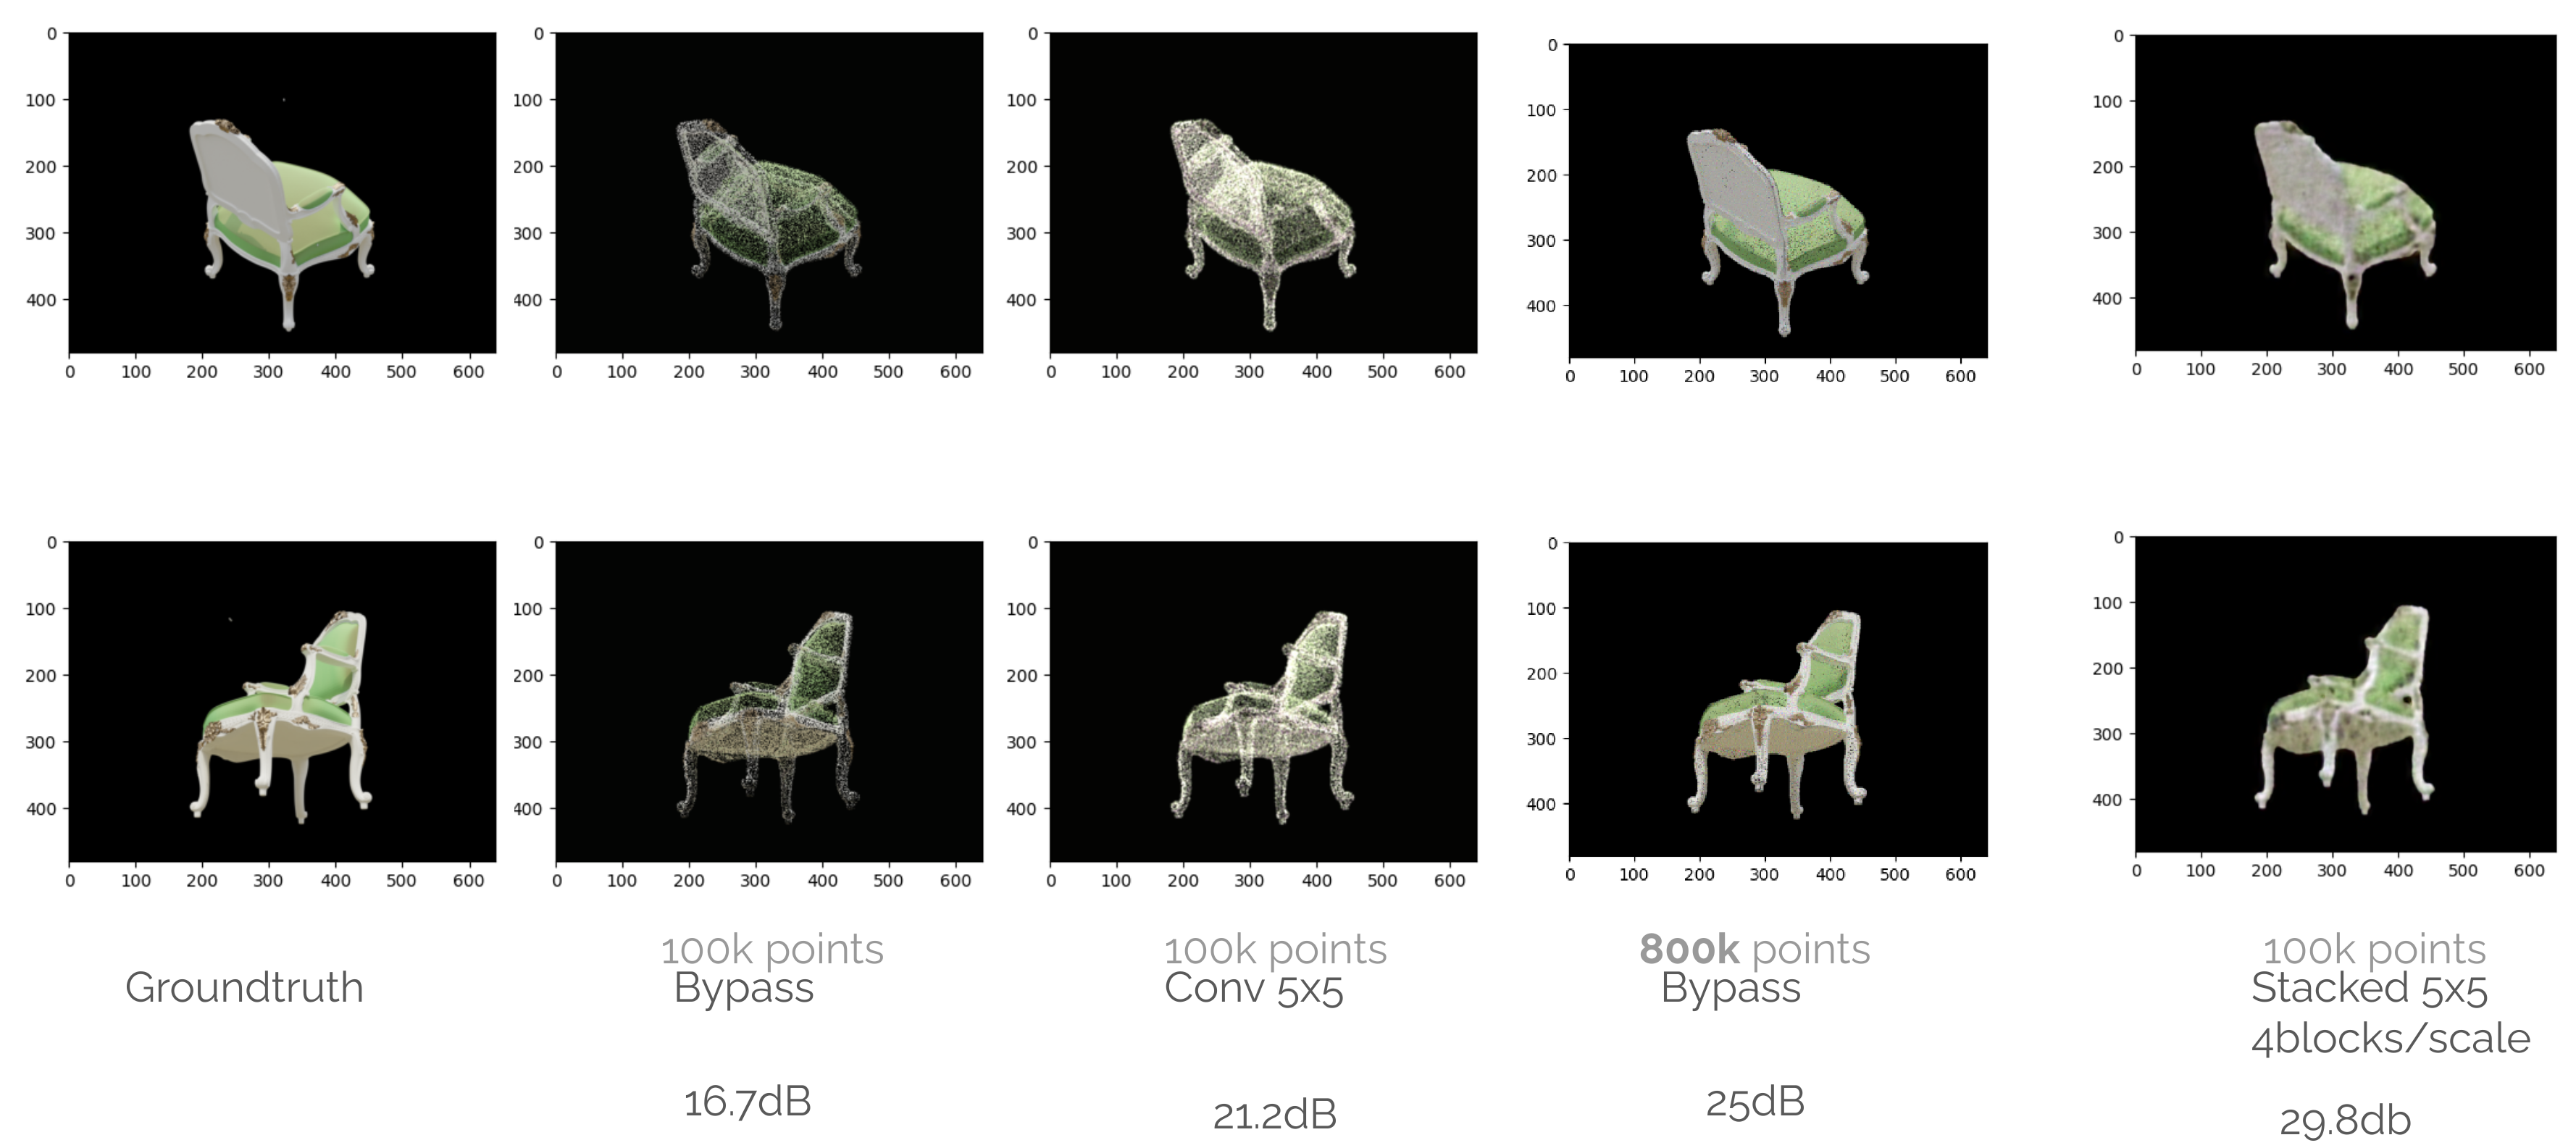
\includegraphics[width=0.85\textwidth]{figures/qualitive_results_chair.png}
    \caption{Two validation novel views using various training options (including the "bypass" mode and vanilla multiscale decoders (at each scale, we're stacking several stages of  Conv5x5+Relu)).}
    \label{fig:results_vanilla}
\end{figure*}


% \begin{figure}[H]
%     \centering
%     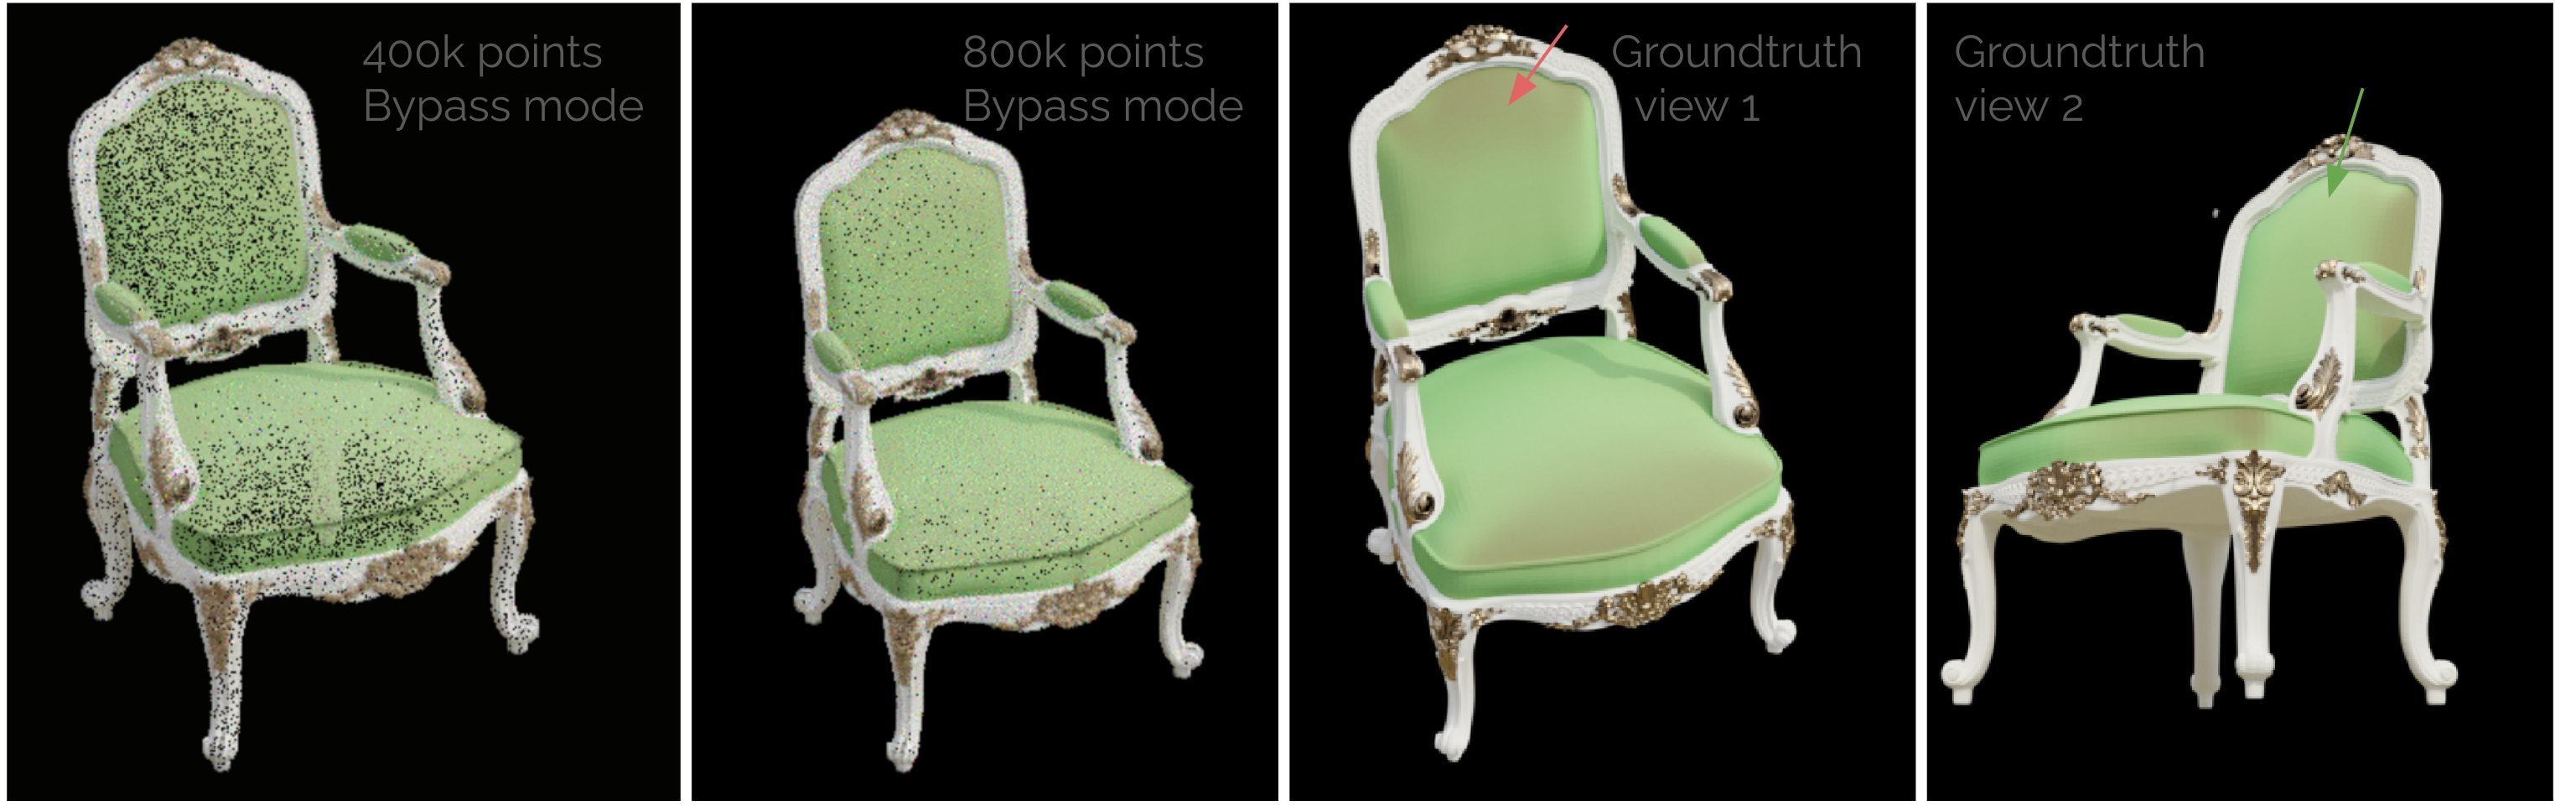
\includegraphics[width=0.45\textwidth]{figures/view_dependancy_issue.png}
%     \caption{View dependant appearance: If we take a careful look at the \texttt{Old chair} scene, we nottice that the foam is slightly shiny in the groundtruth with a red glow on view 1 and a green glow on view 2. No matter how much point we add, we cannot recover this effect with the bypass mode for obvious reasons. It looks like we simply retrieve the diffuse component.}
%     \label{fig:view_dependancy_issue}
% \end{figure}

\begin{figure}[H]
    \centering
    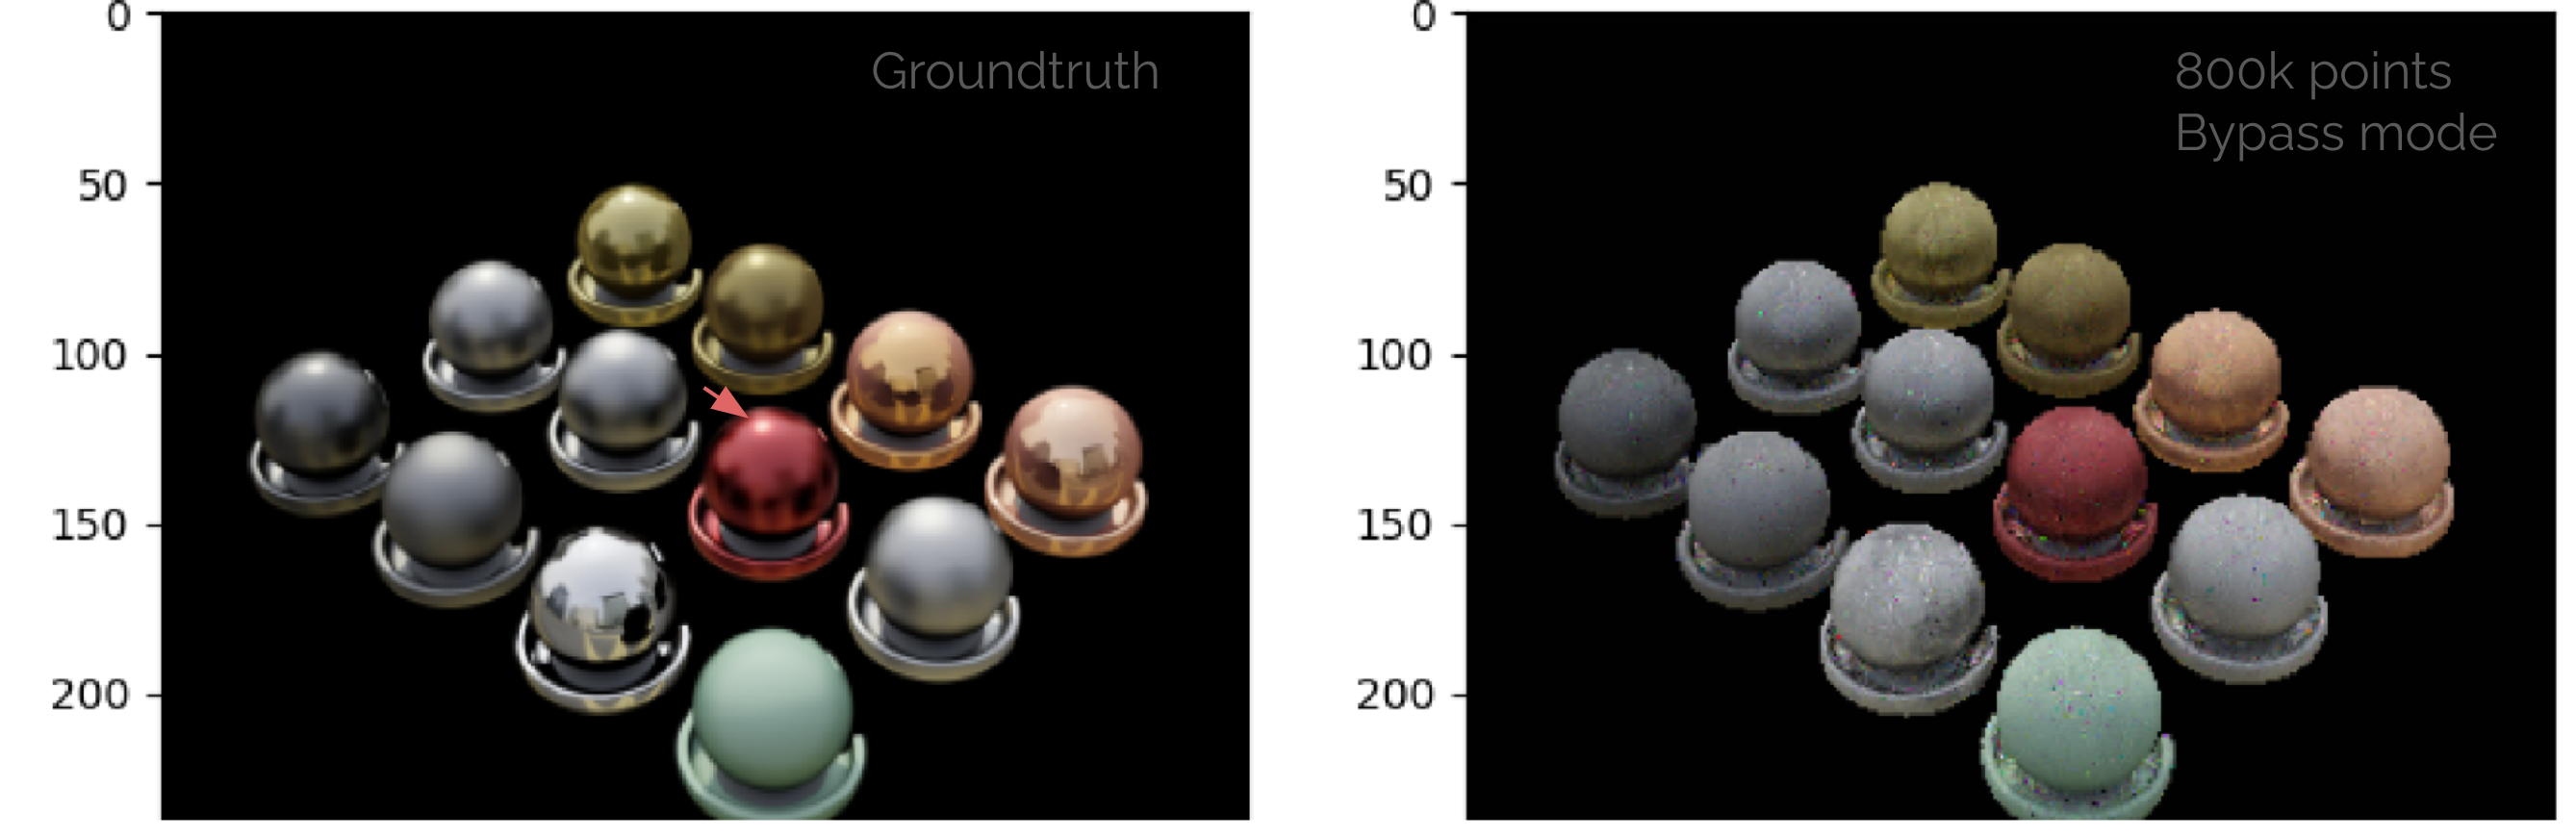
\includegraphics[width=0.45\textwidth]{figures/view_dependancy_issue_mat_balls_arrow.png}
    \caption{View dependant appearance: If we take a careful look at the \texttt{material balls} scene, no matter how much point we add, we cannot recover the view dependancy effect with the bypass mode for obvious reasons. It looks like we simply retrieve the diffuse component. }
    \label{fig:view_dependancy_issue}
\end{figure}

It is not trivial to find a scene with lighting and materials which do not exhibit view dependant appearance, especially it seems like the sample scenes used in the NERF paper were carefully chosen to test the inherent ability of the neural renderer to learn something similar to a BRDF (which models in computer graphics the law of light reflecion for each material, including mirrors)..



\subsubsection{Pixel rendering.}
\label{sec:pixel rendering}
The last operation is to render the final pixel colors by decoding the pseudo color images.
ADOP \cite{ruckert2022adop} and NBPG \cite{Aliev2020} both use a modified UNET \cite{ronneberger2015unet} which is a widely used multi-scale image processing architecture. Two modifications are made to the UNET architecture:
\begin{itemize}
    \item Convolution operator is a gated convolution proposed in a 2019 NVidia paper dedicated to image inpainting \cite{yu2019freeform}. This operator requires knowing the mask (e.g. which pixels are valid).
    \item At each scale, the UNET encoder takes pseudo-colored renders of the point cloud. Note that, at low resolution (higher levels of the pyramid), many points end up being averaged in the same pixel as described in the soft depth test. We end up with thumbnails with not much holes which will intuitively simplify rendering (this is not equivalent to downsampling the full resolution images filled with holes). 
\end{itemize}


\subsubsection{Vanilla networks.}
\label{sec:vanilla rendering}
I started implementing a Vanilla architecture shown in ~\cref{fig:decoders} to make sure I could improve the point cloud rendering right. Due to time constraints, I did not have enough time to implement and train the UNET described in the previous section ~\cref{sec:pixel rendering}.
\begin{figure}[H]
    \centering
    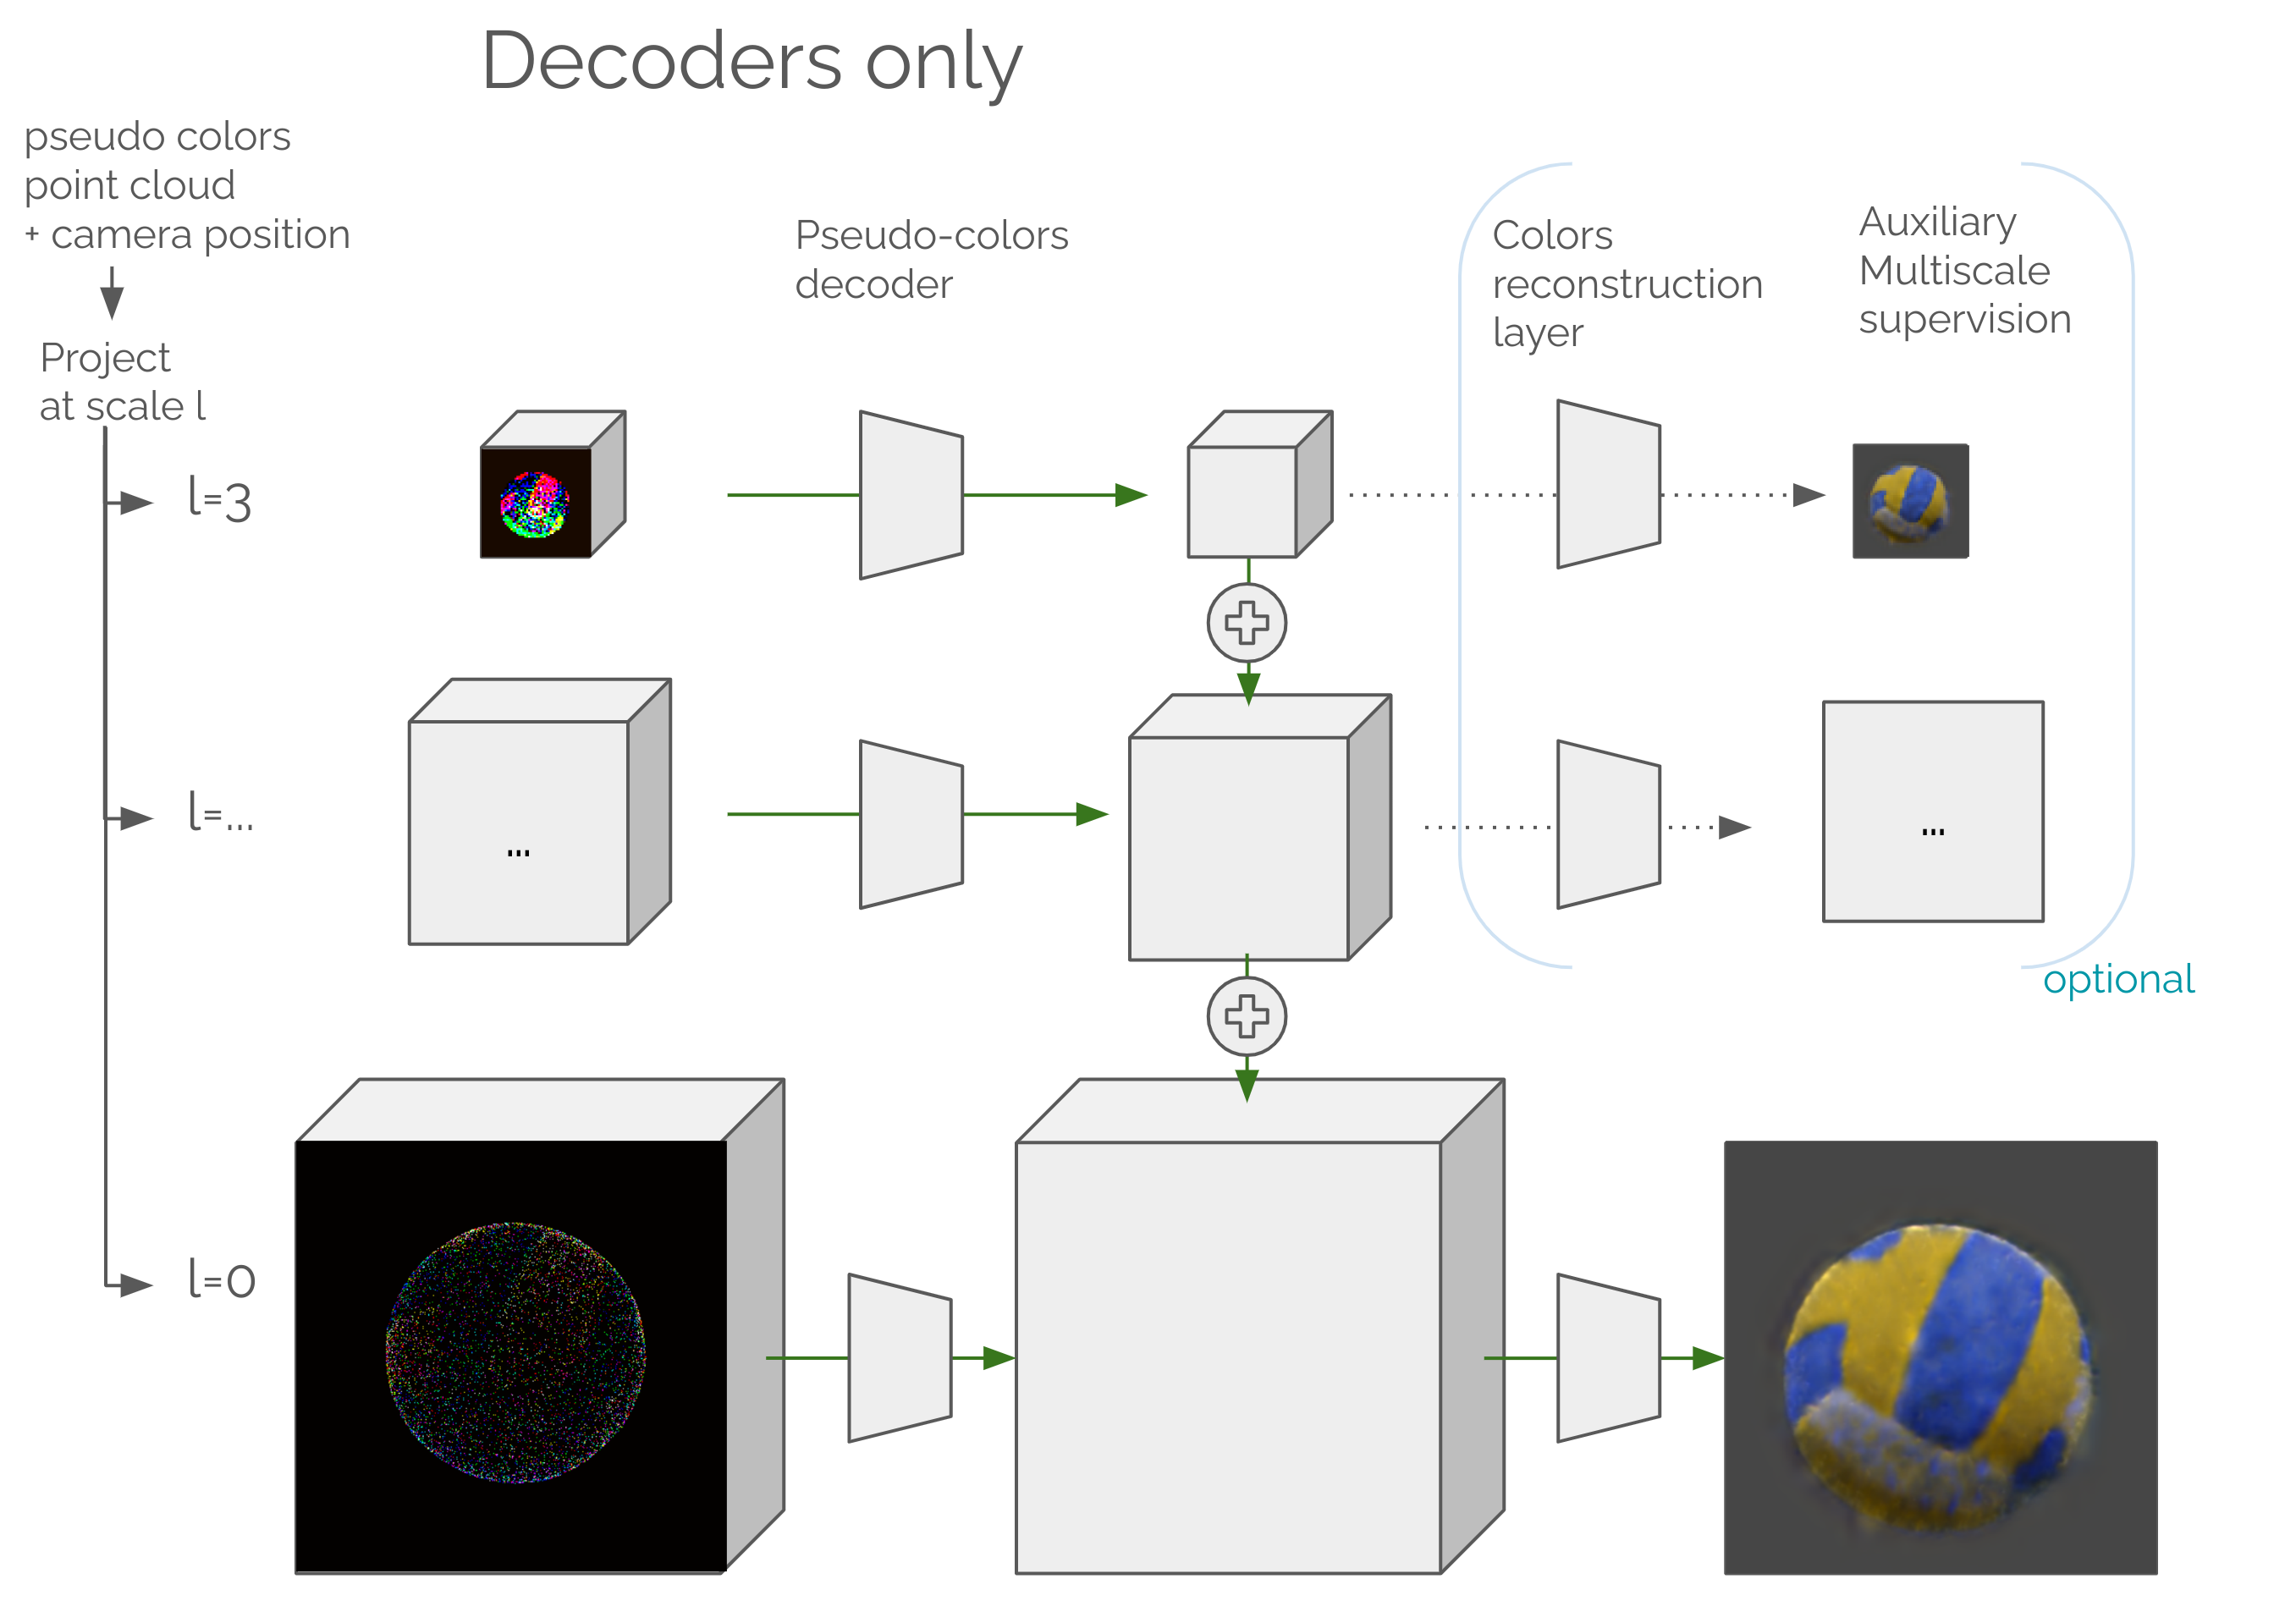
\includegraphics[width=0.45\textwidth]{figures/multiscale_decoders_only.png}
    \caption{Vanilla architecture: Multiscale CNN with decoders only. Pseudo colors have more than 3 channels (4 or 8). At the top of the pyramid ($l=3$), the projected point clould pseudo colors tensor is decoded to a tensor with 8 channels (still not a RGB thumbnail but a feature map). The lower scale $l=2$ will be processed by another decoder - but in a residual fashion (meaning that the decoded feature vector from scale $l=3$ will be upsampled and added to the feature vector of the decoder at scale $l=2$). Finally at scale $l=0$, the high resolution decoded feature map is processed by another Conv+Relu layers to end up with 3 channels. On the right side: an auxiliary decoder at each scale allows to add a potential multiscale supervision loss (not mentioned in the original ADOP paper)}
    \label{fig:decoders}
\end{figure}

We report quantitative performances (PSNR on validation set) of various training configurations on the \texttt{Old chair} scene in ~\cref{tab:results}. By using the CNN rendering on a point cloud of 100.000 points, we're able to "fill the holes" and achieve a better PSNR than the bypass mode with 800.000 points. Qualitively, ~\cref{fig:results_vanilla}, shows blurry results when using the Vanilla architecture. More work is needed to improve the results and implement the UNET architecture with the right parameters.

\textit{Please note that all trainings were performed on a laptop with a Nvidia T500 GPU with only 4Gb of RAM. We decrease the batch size to 8 images when increasing the size of the architecture}.

\subsubsection{Results visualization.}
It is possible to render novel views interactively and live. Please refer to ~\cref{fig:live_inference}.